\documentclass[12pt,a4paper,twoside,nobind]{ociamthesis}

\usepackage{array} 
\usepackage{placeins}
\usepackage[utf8]{inputenc}
\usepackage[T1]{fontenc}
\usepackage[version=4]{mhchem}
\usepackage[position=b]{subcaption}
\usepackage{multirow, mathrsfs, nth, graphicx, amsmath}
\usepackage{helvet}
\usepackage{caption}

% \DeclareCaptionFont{blah}{\footnotesize\fontfamily{\sfdefault}\selectfont}
\DeclareCaptionFont{blah}{\footnotesize\fontfamily{cmss}\selectfont}
\captionsetup{font=blah}
\usepackage{booktabs}
\usepackage[print-unity-mantissa=false,range-phrase=--,range-units=single]{siunitx}
% \usepackage[backgroundcolor=white,
%             textsize=footnotesize,textwidth=2cm]{todonotes}
\usepackage[backend=bibtex,style=chem-acs]{biblatex}
\addbibresource{references.bib}
\renewcommand*{\bibfont}{\footnotesize}
%\AtBeginBibliography{\vspace*{-1cm}}

\newcommand{\ind}[1]{\mathrm{#1''\!\!}}
\newcommand{\direct}[1]{\mathrm{#1'\!}}

\graphicspath{ {figures/} }
\DeclareGraphicsExtensions{.png}

% \newfloatcommand{capbtabbox}{table}[][\FBwidth]
% \floatsetup[ffigbox]{capposition=bottom}
% \newcommand\MyBox[2][red!70!black]{{%
%   \setlength\fboxsep{0pt}\fcolorbox{#1}{white}{#2}}}

\newcommand{\fillcaption}[1]{ %new command with the argument being the text of the caption
	\textbf{Figure \arabic{figure}:} #1 %Makes main figure number, concatenates it to legend
	\addtocounter {figure} {1} %increments main figure count
} 

\setlength{\marginparwidth}{2cm}

\title{Data-driven design of interatomic potentials for metastable chalcogenides}
\author{Joe Morrow}
\college{The Queen's College}
\degree{Transfer of Status Report}
\degreedate{August 2022}

\begin{document}
\setlength{\textbaselineskip}{26pt}
\setlength{\frontmatterbaselineskip}{17pt plus1pt minus1pt}
\setlength{\baselineskip}{\textbaselineskip}
\setlength{\baselineskip}{\singlebaselineskip}
%
% The level that gets a number for ToC:
\setcounter{secnumdepth}{2}
% The level that shows up in the ToC:
\setcounter{tocdepth}{2}
%
\begin{romanpages}
%
\maketitle
%
% \begin{acknowledgements}
%     \input{acknowledgements}
% \end{acknowledgements}
%
\begin{abstract}
The goal of this research is first to understand and second predict the properties
of useful materials by means of computer simulations. One example is the capacity
of a material to store and transport lithium, which determines
the life and maximum electrical power of a battery made from it.
% Specifically, this research will develop Machine Learning (ML) approaches to materials
% modelling, which falls under the EPSRC area of ``manufacturing the future with
artificial intelligence''. 
ML is the science of computer algorithms that
improve with experience, not the explicit intervention of a human programmer.
Modern computer simulations of chemical systems can be highly accurate, whether
in predicting useful properties such as Lithium capacity or unravelling the structure of
complex crystals. However, the simulations usually involve solving (approximately)
the equations of quantum mechanics, which requires prohibitively large computing
power for models that exceed roughly 1000 atoms in size. We develop methods
that ``learn'' from quantum-mechanical data to reach that same level of accuracy
in simulations, but with far less computing time. This provides
access to length-scales in simulations that correspond much more
closely to the situation in real devices, giving us new insights to
design and discover better materials.

One of the main themes of the project is the construction of the training
database: a set of example chemical compounds that the ML models
generalise from to predict the properties of new compounds. We will examine
the following questions:

\begin{itemize}
\item What kind of data is required for sufficient learning? 
% Is it enough to show the
% model lots of disordered liquid atoms for it to
% generalise to all the possible situations an atom might find itself in, or are e.g. solid crystals important too?

\item Training data typically includes hundreds of thousands of examples
of atoms in different environments. How do we evaluate their
information-content systematically? 
% This is important
% because computer memory limitations restrict the number of
% data points that can be used directly for learning, so we must
% select a subset—ideally the most informative ones.

\item How do we tell how accurate the ML model is? It is simple to
compare the force on an atom predicted by the model versus the training data, which gives us one measure of the error of the model. However, this error does not seem to correlate well with that of predictions of properties of the bulk material, e.g. how well
it conducts heat. We likely to be interested in such properties to
design a useful material, so it is important that we have confidence in the
values we calculate for them.
\end{itemize}

As a test case for the ML methods development, we will also study the compounds of the elements Molybdenum and Sulfur. The reasons for choosing these compounds in particular are twofold. Firstly, they are used extensively in the chemical industry as a lubricant, to remove the sulfur from crude oil, and to capture Mercury fumes to stop them escaping into the
environment. More recently, Lithium has been found to move
freely between the sheets of their layered structure, enabling applications in battery
materials. 
% The many uses of Molybdenum Sulfides alone makes understanding and predicting the relationship between their structure and properties important.
Secondly, there has been debate among scientists since the 1970s over the
true structure of MoS3: whether the Molybdenum atoms arrange themselves in
triangles or in long chains. Because of the complexity of the disordered network
formed by these units, the available experimental
evidence is open to interpretation. Computational studies have been
able to provide only limited assistance to date in understanding the experimental
results because they cannot use models with enough atoms to correspond well to
reality. We hope that the new ML methods will be able to resolve the conundrum, in the
process proving both their accuracy and utility.
    % \input{abstract}
\end{abstract}
%
%\dominitoc % decide if you want mini ToC (probs not necessary)
%\dominilof
%\dominilot
\flushbottom
\tableofcontents
%
% \listoffigures
%
% \input{abbreviations}
%
\end{romanpages}
%
\chapter{Nature and aims} \label{chap:introduction}
%

\section{Introduction}
The research for my DPhil thesis centres around the construction of Machine Learning (ML) interatomic potentials
for use in materials chemistry simulations. ML is a group of techniques for extracting useful information from large datasets
with minimal prior knowledge of any laws underlying the data. 
For our purposes, this data is quantum-mechanical energy and force computations on collections of atoms.
By learning from data, 
an ML potential seeks to accurately approximate the quantum-mechanical potential energy surface (PES) in relevant regions of configuration space.
Since the ML potential function is computationally cheaper to evaluate for a given structure by a factor of around \num{e6},
 near-quantum-mechanical quality can be achieved for simulations on far longer timescales and lengthscales.

 \begin{figure}[ht]
  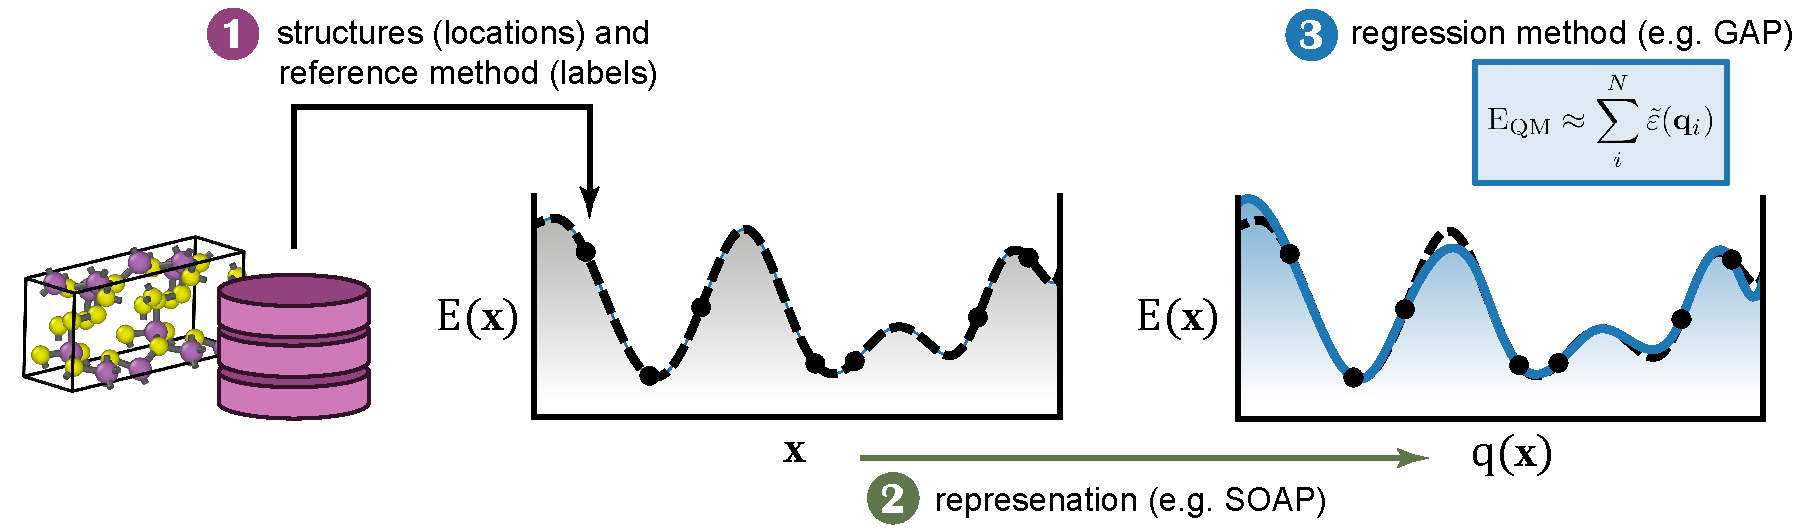
\includegraphics[width=\linewidth]{ML_schematic.pdf}
  \caption{
  Machine Learning interatomic potentials. \textbf{1} Building the database, which consists of structural snapshots (black dots) that sample the PES (dashed line). 
  ``Structures'' here means Cartesian coordinates along with QM forces and a total energy for each entry.
   \textbf{2} The representation: a mathematical encoding of xyz coordinates convenient for learning. This is usually a vector representing the local environment of each atom,
   which is invariant to translations, rotations, and permutations of atoms.
    \textbf{3} Fitting the data. The QM total energy is decomposed into atomic contributions, which are a function of the local environments, and regression performed to minimise the
    error in energy/force predictions on the training database. 
  }
  \label{fig:ML}
\end{figure}

The 3 primary ingredients that go into producing a potential are outlined in Fig.\ \ref{fig:ML}.
Step 1 is building the database:
devising and selecting appropriate structures with enough chemical information to inform the fit,
and calculating the energies and forces of these structures with an accurate reference method (typically DFT).
Step 2 involves encoding the 
local environment of atoms in the database in a mathematical form that is convenient for step 3: the fitting of a flexible function to the reference data.

While I focus primarily on the development of step 1, understanding and practicing steps 2 and 3 are also of critical importance for the performance of the resulting potentials.
There are a number of existing frameworks for 2 and 3, which have been demonstrated to be highly successful in, for example,
describing reactive organic molecules\autocite{Ko2021a}, providing a general purpose model for elemental phosphorus\autocite{Deringer2020c}, and for high entropy alloys.\autocite{Kostiuchenko2019} 
Two methods of particular interest are the Gaussian Approximation Potential (GAP) framework,\autocite{Bartok2010} which employs gaussian process regression as a non-parametric means
to make predictions on ``unseen'' structures based on their similarity to those in the training database,
and the Smooth Overlap of Atomic Positions (SOAP) descriptor,\autocite{Bartok2013} which represents atomic environments as an overlap integral, thereby defining the ``similarity''.

\section{Structural databases and GAP-RSS}

ML potentials have few physical constraints beyond rotation, translation, and permutation invariance.
Therefore, far away from regions sampled in the training database, their predictions are quite likely to be unphysical.
In producing many of the successful general-purpose potentials currently available, choosing the structures to be included in the database was a time-consuming, iterative process.
Early versions of the potential were based on snapshots from \textit{ab initio} Molecular Dynamics simulations (AIMD) to sample high temperature liquid and amorphous phases, and
the known crystalline phases of a material with distortions were added to capture the energy and curvature of minima in the PES. The performance of the resulting potential in predicting the energies
of new structures was then evaluated, and any failings remedied using chemical intuition and trial and error, e.g. adding dimer data to capture the core-repulsion at very short separations,
or adding small-scale models of crystalline defects to enable a better description of similar structures. 

References \cite{Deringer2018} and \cite{Bernstein2019b} describe an alternative approach for exploring the PES in order to build databases.
Instead of adding structures by hand, the principles of random structure searching (RSS), introduced by Pickard \emph{et al.} as a DFT-based crystal structure prediction algorithm,
are employed to automatically sample configuration space.\autocite{Pickard2006,Pickard2011} 
In outline: first, an early version of a potential is initialised on a database of random ``sensible''  structures (i.e. without close approaches of atoms and with some random
symmetry operations). 
Next, this potential is used to relax a new set of random structures to their local minima, a diverse subset of these structures is selected for DFT computations,
and these are added to the database to refit a new potential. 
The previous step is repeated with the latest potential until predictions of satisfactory quality are achieved.

The main advantages of this approach are, firstly, that it is automatic: the most time-consuming step of potential development is the human input of designing the contents of the database,
and, secondly, that it is robust: potentials are prone to predicting spuriously low energetic minima for unseen structures. For an example of such a problem, see the carbon potential\autocite{Rowe2022} which, after publication,
was found to predict body-centred cubic as more stable than graphite. % for a lattice parameter of \SI{2.7}{\text{\AA}}.
Through RSS, sufficient high-energy regions of configuration space, including an unbiased sample of crystal structures, are visited during training to ameliorate the possibility of ``holes'' appearing in the potential's approximation of the PES.
This is important to bound the region explored by a potential during its most common use case: MD simulations.
% 
% define general purpose
%
% \subsection{Amorphous silicon}

\section{Molybdenum Sulfides}

\subsubsection*{Crystalline \ce{MoS2}}
The combination of speed and accuracy offered by ML potentials is most advantageous when applied to systems
where the nanoscale structure is of vital importance.
Crystalline molybdenum disulfide (\textit{c}-\ce{MoS2}) is a well-studied multi-functional material, with properties that 
vary considerably going from bulk to nanoscale.\autocite{Ganatra2014} Consisting of 2D layers of covalently-bound \ce{MoS6} trigonal prisms with weak Van-der-Waals forces acting between layers,
it is simple to exfoliate mechanically, deposit as a thin film electrochemically, and structure into nanoribbons and nanotubes. 

In the bulk it has been used for a long time industrially as a dry lubricant.\autocite{Winer1967}
%\ce{MoS2} is one of the most studied of these, in part because of its ready availability in nature as molybdenite \textbf{Number of papers published on MoS2}.
Nanostructured \textit{c}-\ce{MoS2} is catalytically competent in the hydrogen evolution, hydrogenation, and denitrogenation reactions.\autocite{Tye2006,Wu2013}
\textit{c}-\ce{MoS2} also goes from having an indirect band gap of \SI{1.2}{eV} in the bulk to a direct one of \SI{1.9}{eV} as a monolayer; 
this tunability facilitates its use as a semiconductor for flexible electronics.\autocite{Ganatra2014} 

The relevance of nanoscale structure for the applications of \textit{c}-\ce{MoS2} demands large-scale simulations to fully understand its properties. 
However, the complexity of its open-shell, strongly-correlated 4d electrons and the importance of Van-der-Waals interactions between 
layers also requires a high level of theory to describe accurately, 
which would be too computationally expensive to apply to large unit cells. 
ML potentials are well-placed to offer both, with the means for 
their validation provided by the large body of experimental evidence that is available for this well-studied compound.

\subsubsection*{Amorphous \ce{MoS3}}

The enigmatic compound with stoichiometry \ce{MoS3} %(although the stoichiometry is sensitive to sample origin and history) 
does not crystallise. Instead it remains amorphous (\textit{a}-\ce{MoS3}) or undergoes desulfurisation above \SI{300}{\celsius} to the more-familiar \textit{c}-\ce{MoS2}.
\textit{a}-\ce{MoS3} has attracted interest in research as a less-reactive substitute for elemental sulfur in candidate battery cathodes\autocite{Ye2017} and supercapacitors.\autocite{Pazhamalai2019}
Additionally, its catalytic activity for the hydrogen evolution reaction is superior to that of \textit{c}-\ce{MoS2}.\autocite{Merki2011} 
In spite of this, there remains a decades-old debate concerning the fundamental \ce{Mo-S} structural units contained in \textit{a}-\ce{MoS3}. 
Without clarity on its atomic-scale structure, the details of its catalytically-active sites or lithium migration pathways remain obscure,
whereas they are well-established for \textit{c}-\ce{MoS2}.

\section{Aims}

\subsection*{Validating ML potentials}
Once an ML potential has been trained, the immediate question is to what extent it is accurate and reliable. However, testing the predictions of a potential is not straightforward.\autocite{Zuo2020} Developing robust strategies
for doing so will form a central theme throughout the DPhil research, including:
\begin{itemize}
  \item Physically-guided validation --- testing the predictions of phase transitions by potentials in MD simulations, which is known to be challenging because of the unusual non-equilibrium structures
        that appear along the pathway linking stable phases.\autocite{Deringer2021} 
  \item Numerical errors --- calculating a root-mean-square error in force and energy predictions on a testing set of structures not included during training is the simplest and most common means
        of evaluating a potential. The significance of such a metric depends heavily on which structures are included in the testing set, in particular how diverse they are (it is not challenging to 
        model, with low errors, structures very similar to the known crystalline phases)
\end{itemize}

\subsection*{Fragment-based random structure searching}

The success of RSS-based approaches to fitting ML potentials has been established for single-element systems, but not for multicomponent systems.
Adding additional elements leads to an increase in the amount of data required for training, because \ce{A-A}, \ce{A-B}, and \ce{B-B} interactions (and their many-body analogues, e.g. \ce{A-B-A}) must
be well-represented, instead of only \ce{A-A}. The possibility of charge-transfer and variable stoichiometry also adds to the complexity of designing RSS protocols for multicomponent systems.

It has been proposed that structure searching can be made more efficient when more than one scale of structure
is present in a material by seeding searches with chemical building blocks.\autocite{Ahnert2017, Deringer2018c, Deringer2020}
Using the example of boron: icosahedra can be linked in different ways to produce many near-degenerate crystal structures.
Instead of trying to find the icosahedra from scratch during every search, the smaller configurational space of possible arrangements of entire icosahedral fragments can be explored
much faster.

A major aim of my DPhil research will be the development of heuristics and coding infrastructure for efficient multicomponent RSS,
including the identification of stable, recurring fragments, such as \ce{[MoS6]} trigonal prisms, 
both from structural repositories such as the Materials Project\autocite{Jain2013} and early iterations of RSS.

\subsection*{Understanding amorphous structure}

The combination of speed and quantum-mechanical accuracy allows us to make structural models of amorphous materials that are large enough for a faithful representation of the disorder and accurate on the local scale.
Through, on the one hand, conventional structural-chemical analysis and, on the other, ML-based descriptors and atomic energies, 
my DPhil research aims to provide chemical insight into the principles and driving forces
behind amorphous structure and how we can link the structure to experimental measurements.

\subsection*{Modelling \ce{MoS_x}}

Using the methodological developments described above, I aim to produce a general-purpose ML potential for \ce{MoS_x}.
This will be published openly for others to use in further research into the structures and applications of any material in the \ce{Mo-S} phase diagram.
    
Once the potential is built and validated, I will use it to arrive at a realistic structural model of \textit{a}-\ce{MoS3}
via MD simulations on unprecedentedly large length-scales and in tandem with new experimental diffraction data that I will collect in collaboration with the Goodwin group.
These structural models could subsequently serve as a foundation to understand its Lithium intercalation chemistry and ionic conductivity
 via DFT in the context of battery cathode applications.

%
\chapter{Results and Discussion} \label{chap:theory}
%
\section{Indirect learning}
{\vspace{-2.2em}  \begin{flushright} \small{\emph{(article accepted in J. Chem. Phys)}\autocite{Morrow2022}} \end{flushright}}

Although GAP-based ML potentials are orders of magnitude faster than DFT, alternative ML fitting frameworks exist that are much faster still than GAP,
such as that of the Moment Tensor Potentials (MTP).\autocite{Shapeev2016,Podryabinkin2017}
However, these alternatives typically suffer from poorer extrapolation behaviour compared to GAP models for structures dissimilar to those encountered during training.\autocite{Rosenbrock2021}
In this work, we use an accurate, but more computationally expensive GAP model to generate reference data (locations and labels) for a series of much faster MTP models.\autocite{Morrow2022}
We refer to the idea of using one ML potential to train another with the goal of capturing the original DFT as ``indirect learning''. Figure\ \ref{fig:schematic} outlines the indirect learning concept;
we use the notation $\mathrm{M'}$ for a directly-learned MTP, and $\mathrm{M''}$ for an indirectly-learned one. The ``teacher'' GAP model is taken from Ref.\ \cite{Bartok2018}, namely GAP-18.

\begin{figure}[ht]
  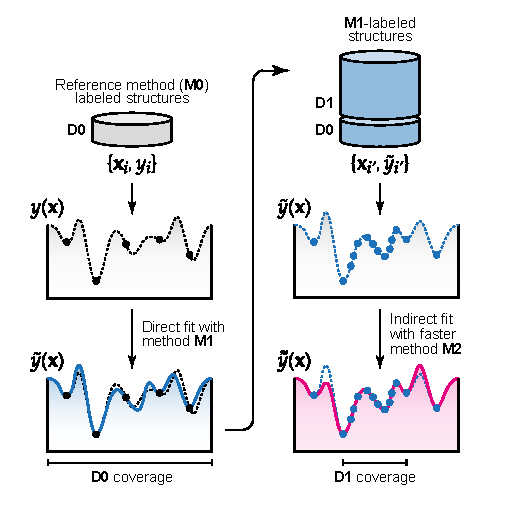
\includegraphics[width=0.6\linewidth]{schematic.pdf}
  \centering
  \caption{
  Indirect learning of interatomic potentials. 
  \textit{Left:} 
  Conventionally, to fit ML potentials, a potential-energy surface is sampled by reference computations
  for a given number of structures, leading to the dataset \textbf{D0}.
  Fitting with the method \textbf{M1} yields an ML potential model (blue line).
  \textit{Right:}
  We now generate a much larger set of structures using \textbf{M1}, and label them using the same method (not \textbf{M0}!).
  This dataset, \textbf{D1}, covers a narrower structural space, but at more points.
  A second fit is then made with a different ML method, \textbf{M2}. Adapted from Ref. \cite{Morrow2022}.
  }
  \label{fig:schematic}
\end{figure}

\begin{figure}[ht]
  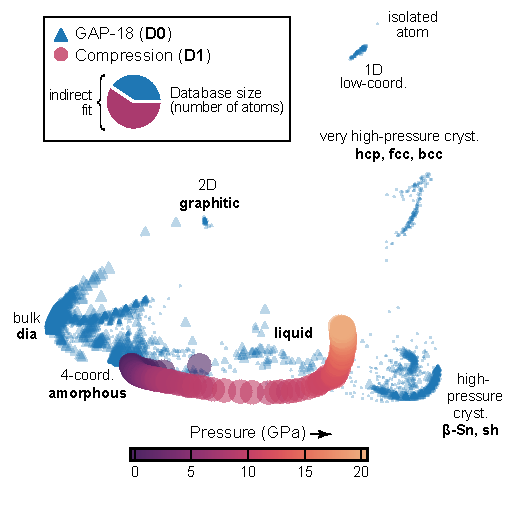
\includegraphics[width=0.6\linewidth]{soap_map.pdf}
  \centering
  \caption{
    Composition of the ML potential fitting databases used in this work.
    A SOAP/KPCA map (cf.\ Ref.\ \cite{Cheng2020}) compares the structural space covered by the GAP-18 database,\autocite{Bartok2018} \textbf{D0}, 
    and the newly created indirect learning dataset, \textbf{D1}. 
    The distance between points on this map is a 2D embedding of their structural dissimilarity as measured by SOAP.\autocite{Bartok2013} 
    At low pressure, a random starting structure, which rapidly transforms to approximate low-density amorphous (LDA) Si, 
    is met with the good coverage provided by liquid and LDA structures in \textbf{D0}. 
    Equally, the high-pressure region is densely sampled with distorted $\beta$-Sn-type and simple hexagonal (sh) structures. 
    However, the \textbf{D0} coverage is distinctly sparse at intermediate pressures around \SI{10}{GPa}.
    The sizes of data points are proportional to the number of atoms in the corresponding training structures, and hence to the number of forces that contribute to fitting.  
    Adapted from Ref. \cite{Morrow2022}.
  }
  \label{fig:soap_map}
\end{figure}

Without the need for additional quantum-mechanical computations, extensive databases can be easily generated with the GAP,
and we find that this improves the quality of fast potentials with less flexible functional forms.
We test the technique on disordered silicon, 
including a simulation of vitrification and polycrystalline grain formation under pressure with a system size of a million atoms.



\section{Application to Silicon}

\begin{figure}[!ht]
  \centering
  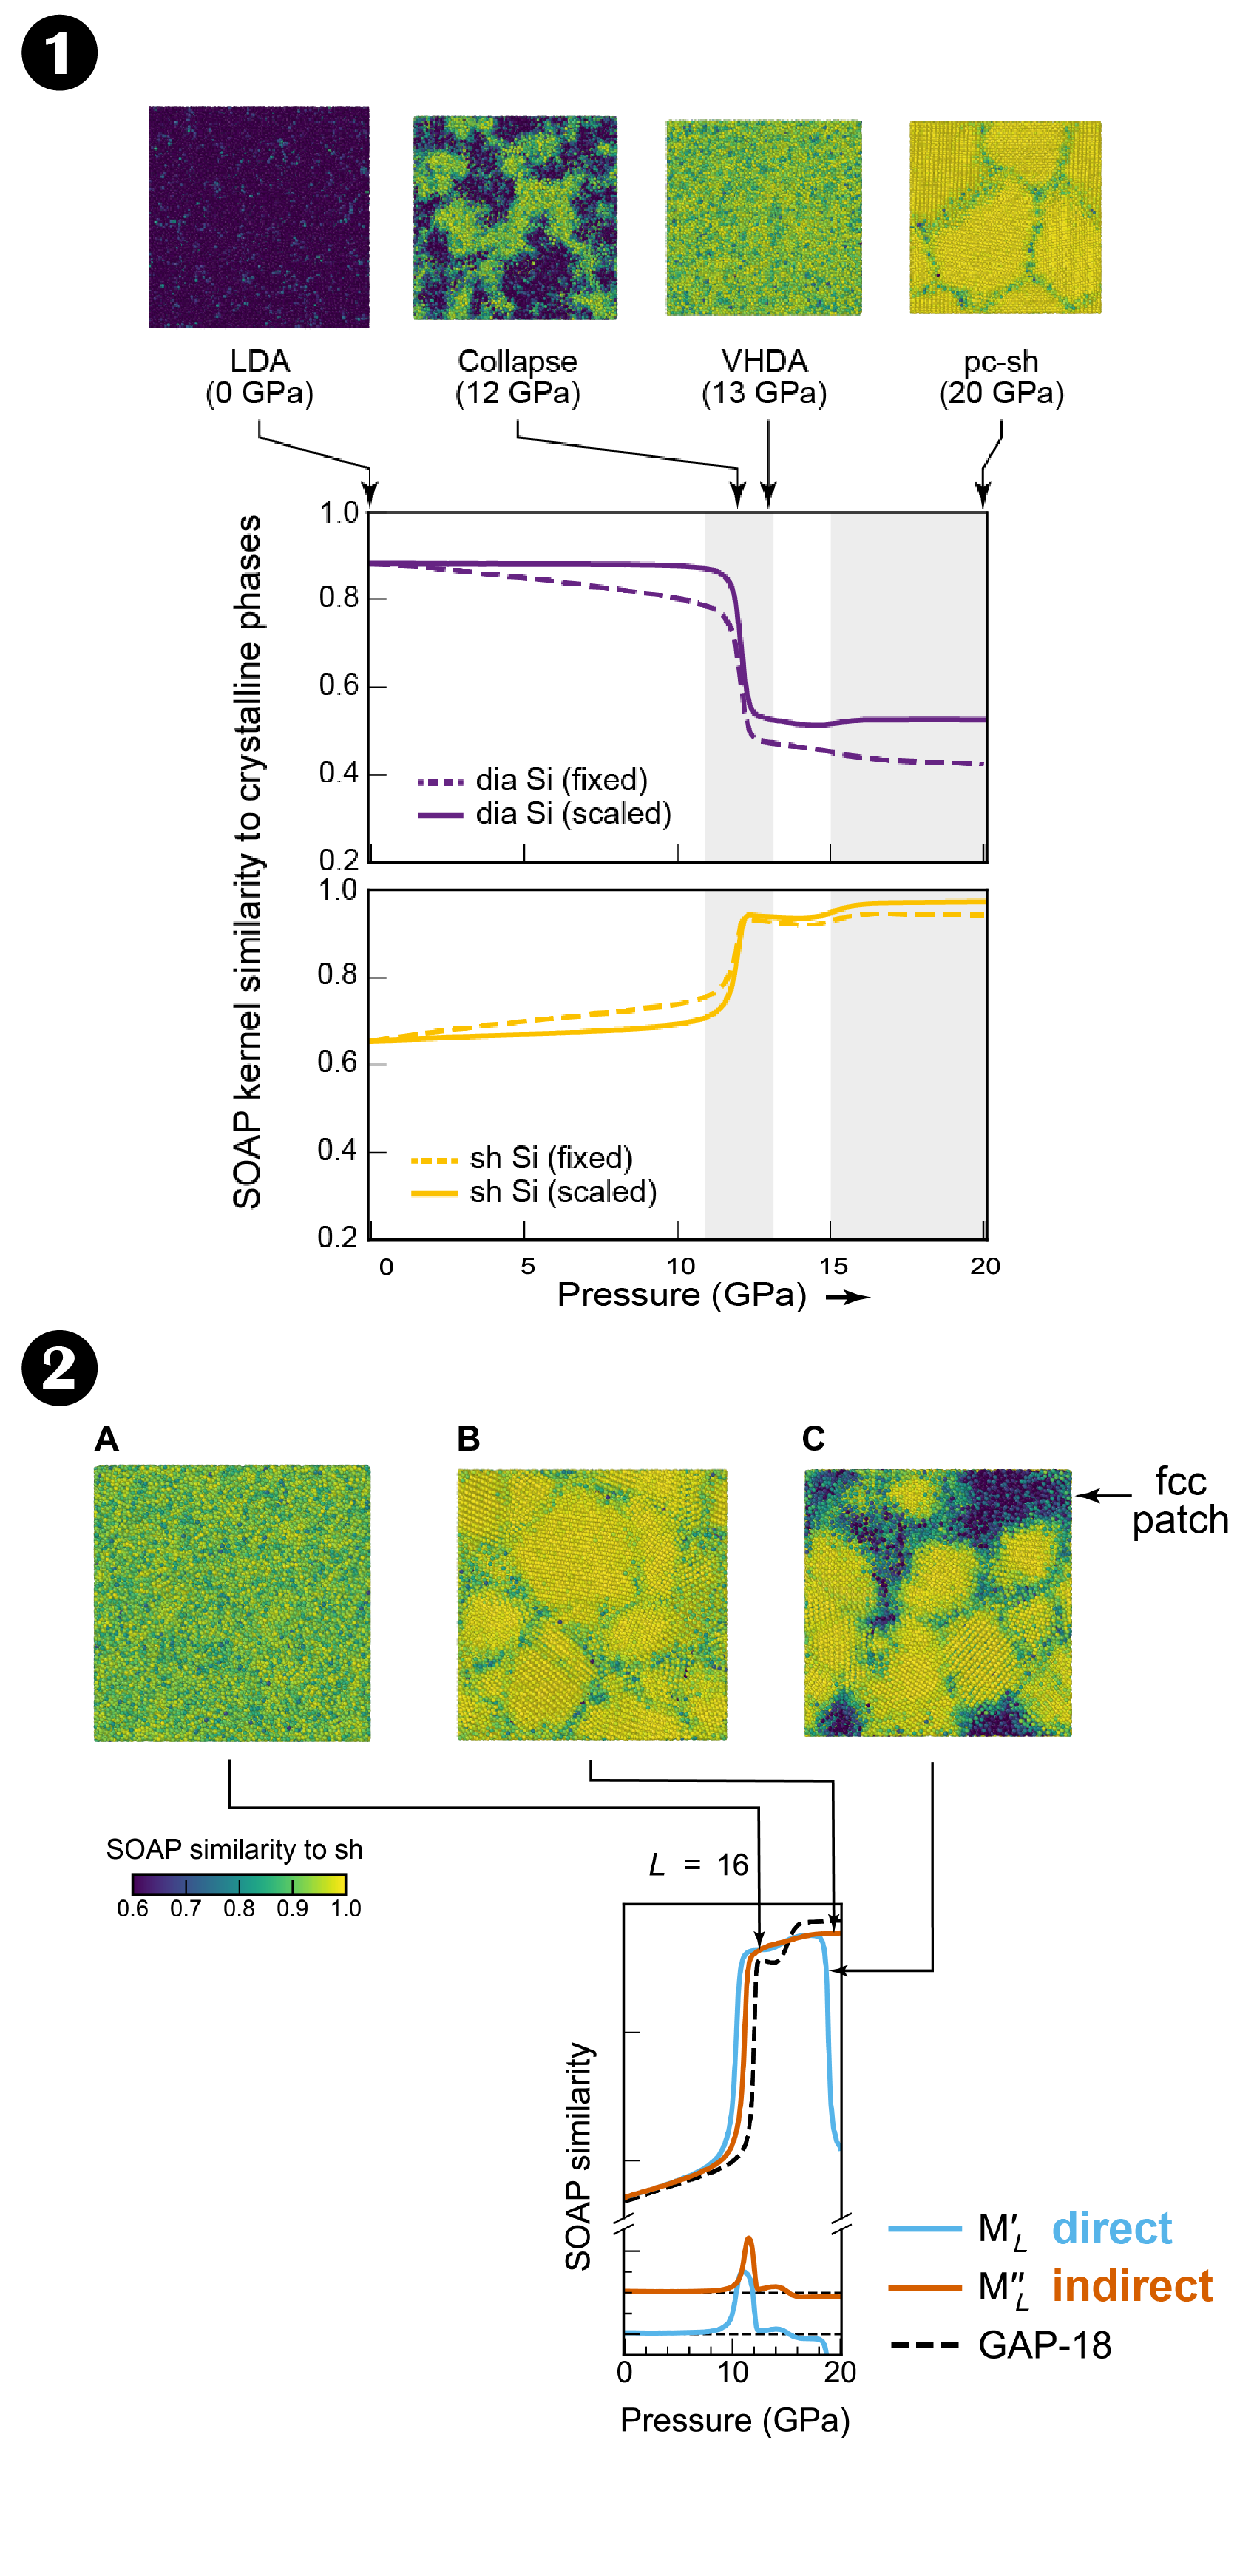
\includegraphics[width=0.5\linewidth]{simplified_compression_series.png}
  \caption{
    \textbf{(1)} A structural benchmark for high-pressure disordered Si.
    We evaluate the average SOAP similarity of the compression trajectory of Ref.\ \cite{Deringer2021} to selected crystalline structures.
    Dashed lines are for reference crystals with a fixed lattice optimised at \SI{0}{GPa} with DFT. 
    Solid lines are similarities to crystals with their lattice parameters optimised as a function of pressure. 
    The structure images show representative snapshots, color-coded according to SOAP similarity to the sh crystalline phase,
    with lighter colors indicating higher similarity.
  \textbf{(2)}%
    Performance of an indirectly-learned model in 100,000-atom compression simulations of amorphous Si.
  We report the average SOAP similarity to pressure-adjusted sh Si during compression (cf.\ Fig.\ S1), benchmarking MTPs (solid) versus GAP-18 (dashed).
  The difference for each MTP to GAP-18 is plotted underneath the absolute values, with $\ind{M}_{L}$ offset.
  Representative snapshots during the run are displayed, colored by atomistic SOAP similarity to sh (\textbf{A}--\textbf{C}). 
  % Points where MD simulations become numerically unstable (for $\direct{M}_{14}$ and $\direct{M}_{20}$) are marked with asterisks.
  }
  \label{fig:SOAP_difference}
\end{figure}

Figure\ \ref{fig:SOAP_difference} summarises the key result of our article.\autocite{Morrow2022} Working towards my aim of developing physically-guided methods to evaluate the performance of potentials,
we use MD simulations with a constant pressure ramp to test whether the potential predicts the experimentally-confirmed series of Si phases.
The SOAP descriptor, as well as functioning as a component of fitting ML potentials, can also be used to render large structural snapshots chemically interpretable.
The SOAP kernel gives the similarity between two atomic environments on a scale from 0 (dissimilar) to 1 (identical up to rotations and translations); in Fig.\ \ref{fig:SOAP_difference} we compare snapshots
from MD trajectories to simple-hexagonal and diamond crystalline phases. In a new development, by adjusting the external pressure experienced by the reference crystal, the comparison is made more
consistent --- e.g. the low density amorphous (LDA) form of Si, which is most similar to diamond, remains at a constant similarity to diamond before the sudden structural collapse at \SI{12}{GPa}, 
which reflects the fact that pressurisation results in a uniform contraction of bondlengths, without structural rearrangement, until the collapse.

Overall, indirectly-learned MTPs perform much more reliably at the compression test than those directly fitted (to \textbf{D0}), 
with every $\ind{M}_{L}$ model (a representative one is shown in Fig.\ \ref{fig:SOAP_difference})
producing the expected sequence of phases, viz.\ LDA $\longrightarrow$ very-high-density amorphous (VHDA) $\longrightarrow$ polycrystalline (pc) sh.\autocite{Deringer2021}
Additionally, the indirect MTPs were validated using numerical error measures and other physically-guided tests---including the production of high-quality models of low-density amorphous Si
(see Table\ \ref{tab:LDA}, where the parent model, GAP-18, can be taken as a benchmark for the state-of-the art in modelling \emph{a}-Si).

\begin{table}[ht]
  \centering
  \caption{Quality metrics for 100,000-atom LDA Si models produced by \SI{e11}{K s^{-1}} quench simulations: proportion of 3- and 5-fold connected atoms ($N_{3}$ and $N_{5}$),
  determined using a cutoff of \SI{2.85}{\text{\AA}}; inverse height of the first sharp diffraction peak ($H^{-1}$);
  \autocite{Xie2013} mean ($\bar{\theta}$) and width ($\Delta \theta$) of the bond-angle distribution; 
  and energy above diamond-type Si calculated with GAP-18.
  }\label{tab:LDA}
  \begin{tabular}{l
  S[table-column-width=1.2cm, round-mode=places, round-precision=2]
  S[table-column-width=1.2cm, round-mode=places, round-precision=2]
  S[table-column-width=1.4cm, round-mode=places, round-precision=3]
  S[table-column-width=1.4cm, round-mode=places, round-precision=2]
  S[table-column-width=1.4cm, round-mode=places, round-precision=2]
  S[table-column-width=1.4cm, round-mode=places, round-precision=3]} \toprule
      \centering
       {Model} &   {$N_{3}$ (\%)} & {$N_{5}$ (\%)} & {$H^{-1}$} & {$\bar{\theta}$ (deg)} & {$\Delta \theta$ (deg)} & {$\Delta E$ (\si{eV})}  \\ 
      \midrule \\[-1em]
      $\direct{M}_{16}$   & 0.565     &   2.366       & 0.602664  & 108.99287      & 10.8465  & 0.156473  \\
      $\ind{M}_{16}$      & 0.677     &   1.637       & 0.560067  & 109.14605      & 10.2342  & 0.151846  \\
      \midrule \\[-1em]
      $\direct{M}_{20}$   & 0.471     &   3.645       & 0.498157  & 108.92970      & 10.9086  & 0.146161  \\ 
      $\ind{M}_{20}$      & 0.691     &   1.329       & 0.503525  & 109.16124      &  9.9319  & 0.143802  \\ 
      \midrule \\[-1em]
      GAP-18              & 0.696     &   0.952       & 0.563539  & 109.17405      &  9.9876  & 0.145155  \\
      \bottomrule
  \end{tabular}
  \end{table}


\section{Taxonomy of defects in Silicon}
{\vspace{-2.2em}  \begin{flushright} \small{\emph{(manuscript in preparation)}} \end{flushright}}

The indirect MTPs achieve around a 1000-fold acceleration in the computational time required to run MD compared to GAP-18, whilst maintaining almost the same quality in their description of the PES.
The access to longer lengthscales and timescales enables us to study in detail the structure of coordination defects,
which are embedded at the \SIrange{1}{2}{\%} level in a predominately fourfold-coordinated random network. The decomposition of the total energy into atomic contributions provides a handle with which 
to analyse defect stability and formation. The extent to which ML atomic energies, which are not a quantum-mechanical observables, are chemically meaningful is an open question in the field.
We aim to link these local energies to conventional structural measures to advance the interpretability of ML potentials' predictions. 

 \begin{figure}[ht]
  \centering
  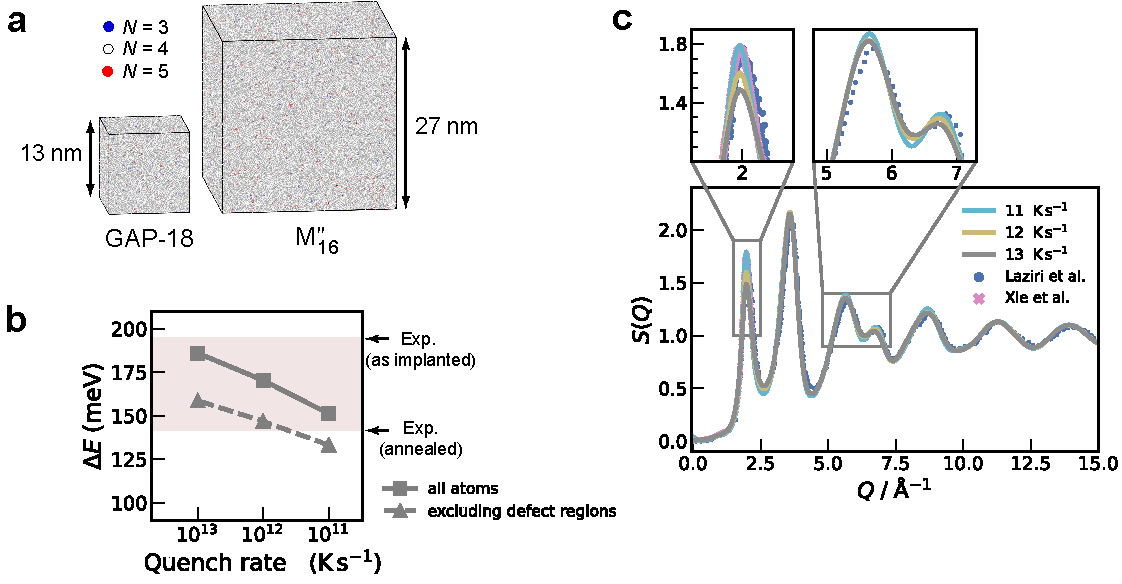
\includegraphics[width=\linewidth]{rejig_fig1_tos.pdf}
  \caption{
  A 1-million structural model of \emph{a}-Si produced with indirectly-learned potential. \textbf{(a)} Size comparison for models
  obtained by melt-quenching at \SI{e11}{Ks^{-1}} to \SI{500}{K} before relaxation. Color-coding indicates coordination numbers, $N$. 
  \textbf{(b)} Excess energy per atom of the 1-million atom model of \emph{a}-Si vs. diamond-type Si, as a function of quench rate. Solid lines show averages over all atoms, 
  dashed lines exclude coordination defects and their neighbouring atoms.
  Pink shading denotes the region of energy consistent with experiments.\autocite{Roorda1991}
  %
  \textbf{(c)} Structure factors for varying quench rate compared to experiments.\autocite{Laaziri1999,Xie2013}
  }
  \label{fig:defects1}
\end{figure}

\begin{figure}[ht]
  \centering
  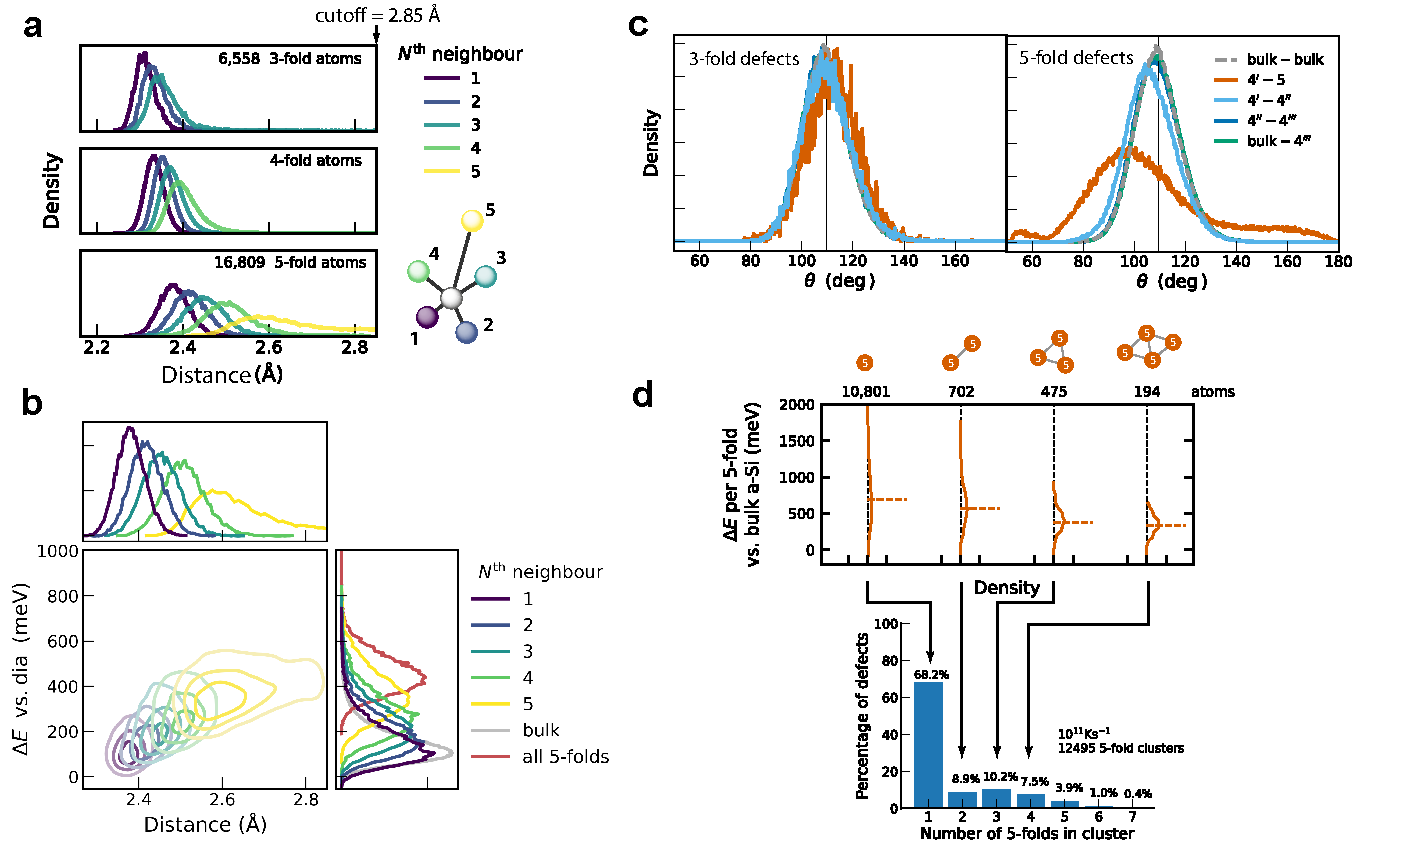
\includegraphics[width=\linewidth]{rejig_fig2_tos_2x2.pdf}
  \caption{
    Local structural and energetic analysis of defects. 
    \textbf{(a)} $N^{\mathrm{th}}$-nearest neighbour histograms for 3-fold, 4-fold, and 5-fold coordinated atoms separately, where atoms are defined as bonded if closer than \SI{2.85}{\AA}.
    For each atom in the structure, its $N$ nearest neighbours are sorted by bond length and these bond distances added to separate histograms.
    %
    \textbf{(b)} Correlation between ML atomic energy and bond distance for 5-fold coordinated atoms. Similar to \textbf{a}, 
    we plot the distance histograms of nearest neighbours on the horizontal axis, and histograms of their corresponding atomic energies on the vertical axis. For reference, the atomic energy histograms
    of all 5-fold atoms (red) and all 4-fold atoms in the bulk (grey) are included.
    %
    \textbf{(c)} Bond angle distribution functions (BADFs) in the neighbourhood of 5-fold (left) and 3-fold (right) coordination defects.
    In the legend, 3 refers to 3-fold atoms, 5 to 5-fold atoms, 4$^\prime$ to 4-fold atoms one bond away from a corresponding defect, and 4$^{\prime\prime}$ to one two bonds away etc. 
    `Bulk' refers to angles in the non-defective regions of the structure, i.e. any 4-fold atoms further than 3 bonds away from any defect centre.
    Bonded triples are amalgamated to condense information such that, for example, 4$^\prime$ – 5 refers to all triples involving atoms of the type 4$^\prime$ and 5 and no others.
    %
    \textbf{(d)} Atomic energy distributions for the most common defect clusters, left to right.
    The bar chart (lower) reports statistics on the clustering of coordination defects. 
    }
  \label{fig:defects2}
\end{figure}

In Fig.\ \ref{fig:defects1}, we characterise the bulk properties of a very-large structural model of LDA Si produced via melt-quench simulations.
Slower quenching leads to a higher first sharp diffraction peak (FSDP) as has been observed previously;\autocite{Deringer2018d} the most slowly quenched (\SI{e11}{Ks^{-1}}) model shows near-perfect agreement with the experimental $S(Q)$.
The excess energies also decrease with quench rate, which indicates a more relaxed amorphous network. The number of defects also decreases substantially with quench rate (7\% to 2\%).
However, the majority of the stabilisation gained by slower quenching is associated with relaxation of the `non-defective' regions of the structure, 
which is evidenced by the near parallel decrease of the non-defective atomic energies with quench rate compared to the total atomic energies.

Figure\ \ref{fig:defects2} illustrates the results of a local analysis of the structure of defects. 
Histograms are left unsmoothed throughout, which emphasises the high level of statistical significance available to us due to the large system size.
In Fig.\ \ref{fig:defects2}a, as coordination number lowers, so do the typical distances between bonded atoms---as is widely observed throughout structural chemistry.
The definitive \nth{5} peak and even spacing between peaks for the 5-fold distribution indicate that a majority of such defects are best described as `truly' 5-coordinate, rather than [4+1]. 
The longer tail in the \nth{5} peak contains the minority of distant \nth{5} neighbours. 
There is a strong correlation between the bond distance to a neighbour and that neighbour's local energy (see Fig.\ \ref{fig:defects2}b)

In Fig.\ \ref{fig:defects2}c, angles involving 5-fold atoms deviate substantially
from the ideal tetrahedral angle and have a very broad distribution. 
The structural disturbance associated with these defects persists to the next-nearest bonds between 4$^\prime$ and 4$^{\prime\prime}$ atoms, 
which have a significantly lower mean angle and broader distribution than that of the bulk.

Although the majority of defects present as isolated over- or under-coordinated atoms, there is a stronger tendency for 5-fold atoms to occur together than can be expected from random placement of defects.
3-folds are much more likely to be isolated. The energy distributions of Fig.\ \ref{fig:defects2}d show that clustering reduces the average excess energy associated with the defect atoms and their immediate neighbours---in a manner akin to reducing surface tension by minimising interfacial area. This is consistent defects having an extended range, where strain is induced in the structure surrounding the core, which is
visible in both the angles distributions and local energetics.


% \section{Synthesis and characterisation of \emph{a}-\ce{MoS3}}

% \section{Random Structure Searching}

%
%
%\begingroup
%\let\clearpage\relax
%\vspace{60pt}
\chapter{Future work}

% \section{Further applications of indirect learning}

\section{Modelling of a-\ce{MoS3}}

With assistance from Dr.\ Simon Cassidy (Clarke group), we have carried out trial syntheses of \textit{a}-\ce{MoS3} via thermal decomposition of \ce{(NH4)_2MoS4} under argon. 
Characterisation via Raman spectroscopy, powder diffraction, and ICP-MS
is continuing (currently in early stages). 
We have been awarded beam time for the POLARIS instrument at ISIS to collect neutron total scattering data. 
With the corresponding X-ray data to provide contrast between Mo and S, we plan to derive
a high-quality experimental pair-distribution function, against which we can directly compare large-scale structural models produced via ML-driven simulations.


On the modelling side, I have developed a GAP-RSS framework in \texttt{Python}, which will make publically available after testing later in the DPhil. I am beginning to apply this framework to building a potential for the Mo--S phase diagram.
Early version of the potential are showing encouraging results in MD simulations (see Fig.\ \ref{fig:MoS2} for an example of disordered \ce{MoS2} produced via melt-quench simulations). 

\begin{figure}[ht]
  \centering
  \includegraphics[width=0.7\linewidth]{MoS2.pdf}
  \caption{
    Snapshot from a 1000-atom melt-quench simulation of \ce{MoS2}, driven by an early RSS-based GAP model. Poorly-crystalline, intergrown layers of \ce{[MoS6]} trigonal prisms can be observed.
    }
  \label{fig:MoS2}
\end{figure}

In future work, I will develop a series of chemically-motivated tests
 for the potential, for example the layer exfoliation energy, layer-slipping, and layer-twisting barriers. 
 These will form an important part of validating the potential. 
 I will also use such tests, along with numerical error measures,
 in a study of the effect of the GAP-RSS design choices on the kind of structures searched, and the performance of resulting potentials. 
 At this stage, introducing fragment-based seeding of searches and more advanced structure selection algorithms will
 provide further opportunities to tune the RSS.

 With a high-quality \ce{MoS_x} potential constructed, I will move on to large-scale modelling of \ce{MoS3}, which may require methods beyond simple MD, such as enhanced sampling, 


\section{Further applications of indirect learning}

In collaboration with other members of the Deringer group, I plan to apply the concept of indirect learning, which we established works well for Si, to other accurate but expensive GAP models, such as the general-purpose phosphorus potential
of Ref.\ \cite{Deringer2020} and the Ge-Sb-Te (GST) potential of Ref.\ \cite{Zhou2022} for phase-change materials. If successful, the accelerated versions of these potentials will enable, for example, a more detailed study of the liquid--liquid phase
transition of phosphorus, and device-scale simulations of repeated switching between amorphous and crystalline phases for GST.

%\endgroup

\clearpage
%
% \setlength{\baselineskip}{0pt}
% \renewcommand{\abovechapterskip}{\vspace*{-10pt}}
\printbibliography

%
\clearpage
\startappendices
\small
\section*{Transferable skills}
\begin{itemize}
  \item Time management: I have been managing multiple projects, lab work, Part II projects, teaching, and collaborations simultaneously.
  \item Graphic design: for making attractive figures using Adobe Illustrator.
  \item Coding: I have learned new languages (Fortran, Julia) and substantially improved skills, e.g. version control
  \item Presentation skills: the OxICFM CDT taught course involved plentiful opportunities to present to an audience, as has the group meetings that come with being a member of two research groups (Deringer and Goodwin).
  \item Teamwork: the OxICFM CDT taught course involved team presentations and tasks. I have also participated in a group project on best practice and benchmarking for DFT calculations.
\end{itemize}

\section*{List of lectures and seminars}

\begin{itemize}
  \item 15/02/21; Prof. Tomislav Friščić (McGill University); Green Chemistry in the Solid State: Sky is the Limit
  \item 12/10/21;	Prof. M. Stanley Wittingham (Binghamton);	The Lithium Battery, from a Dream to Readiness to take on Climate Change – Opportunities and Challenges
  \item 19/10/21;	Prof. Ludmilla Steier (Oxford);	Material Design Strategies for Solar Fuel Production
  \item 29/10/21;	Prof. Sarah Bostrom (Oxford);	Microwave Catalysis and Prussian Blue Tilting
  \item 23/11/21;	Prof. Christoph Salzmann (UCL);	Complex materials: From hydrated hydrophobes and pink phosphorus to stacking-disordered silver iodide
  \item 30/11/21;	Prof. Leslie Schoop (Princeton);	The Chemistry of Quantum Materials
  \item 10/12/21; Dr. Kasper Tolborg (Imperial College London); Computational modelling of entropic stabilisation in inorganic and hybrid materials
  \item 10/12/21; Bradley Sheath (Oxford); Magnetic ordering on the transition metal sub lattices of Sr2Cr3O3As2 and related compound
  \item 14/02/22;	Prof. Fernanda Duarte (Oxford);	Exploring chemical reactivity with machine learning and automation
  \item 23/02/2022; Dr Tim Green (DeepMind, Google); Highly accurate protein structure prediction with AlphaFold, and AI for quantum chemistry
  \item 06/05/22; Prof. John Hu (West Virginia University); Electromagnetically Initiated Catalysis for the Production of Hydrogen, Ammonia from renewable power, and Chemicals from plastics, natural gas
  \item 06/05/22; John Cattermull (Oxford); Prussian blue analogues for K-ion batteries: a complex structural challenge
  \item 16/06/22; Prof. Jarad Mason (Havard); Manipulating Phase Transitions and Porosity in Metal–Organic Materials: From Solid Refrigerants to Microporous Water
  \item 22/06/2022; Prof. Sebastian Henke (TU Dortmund); Responsive and glassy metal-organic frameworks
  \item GAP Developers' and Users' Meeting, Helsinki, Finland (talk given, 4-9 Aug 2022)
  \item Psi-K Conference, Lausanne, Switzerland (poster given, 22-25 Aug 2022)
  \item DPG Spring Meeting, Condensed Matter Section, Regensburg, Germany (talk given, 4-9 Sep 2022)
\end{itemize}



\section*{MPLS Graduate School courses}
\begin{itemize}
  \item Leading collaboration: bringing people together to achieve the extraordinary
  \item Networking: a systematic approach
  \item Research ideas with enterprise tools: charting it out
\end{itemize}

\section*{Teaching}
\begin{itemize}
  \item Demonstrating for ``Advanced Computational Methods for Solid State Chemistry'' course for OxICFM CDT
  \item Tutorial classes for the Quantum Chemistry supplementary course
  \item Tutorial class in solid-state Inorganic Chemistry for students of The Queen's College
  \item Supervision of Part II student and two TMCS MSc students
  \item Teaching \nth{2}-year Inorganic Chemistry course to Magdalen College students (starting academic year 2022-2023)
\end{itemize}

\end{document}